\documentclass[11pt]{article}

% ---------------- Packages ----------------
\usepackage[margin=1in]{geometry}
\usepackage{amsmath,amssymb,amsthm}
\usepackage{graphicx}
\usepackage{hyperref}
\usepackage{fancyhdr}
\usepackage{enumitem}
\usepackage[UTF8]{ctex}
\usepackage{algorithm}
\usepackage{algpseudocode}
% ---------------- Header ----------------
\pagestyle{fancy}
\fancyhf{}
\lhead{Course Name}
\rhead{Homework \#1}
\cfoot{\thepage}

% ---------------- Title ----------------
\title{Homework 1}
\author{羊瑞 \\ 2300013091}
\date{\today}

% ---------------- Custom commands ----------------
\newcommand{\R}{\mathbb{R}}
\newcommand{\E}{\mathbb{E}}

% ---------------- Problem Environment ----------------
\newcounter{problem}

\newenvironment{problem}[1][]{
\stepcounter{problem}
\section*{Problem \theproblem\; #1}
}{}

\newenvironment{solution}{
\par\noindent\textbf{Solution.}\par\noindent
}{\qed}

\setlength{\parindent}{0pt}
% ---------------- Document ----------------
\begin{document}

\maketitle

\begin{problem} 
\begin{center}
    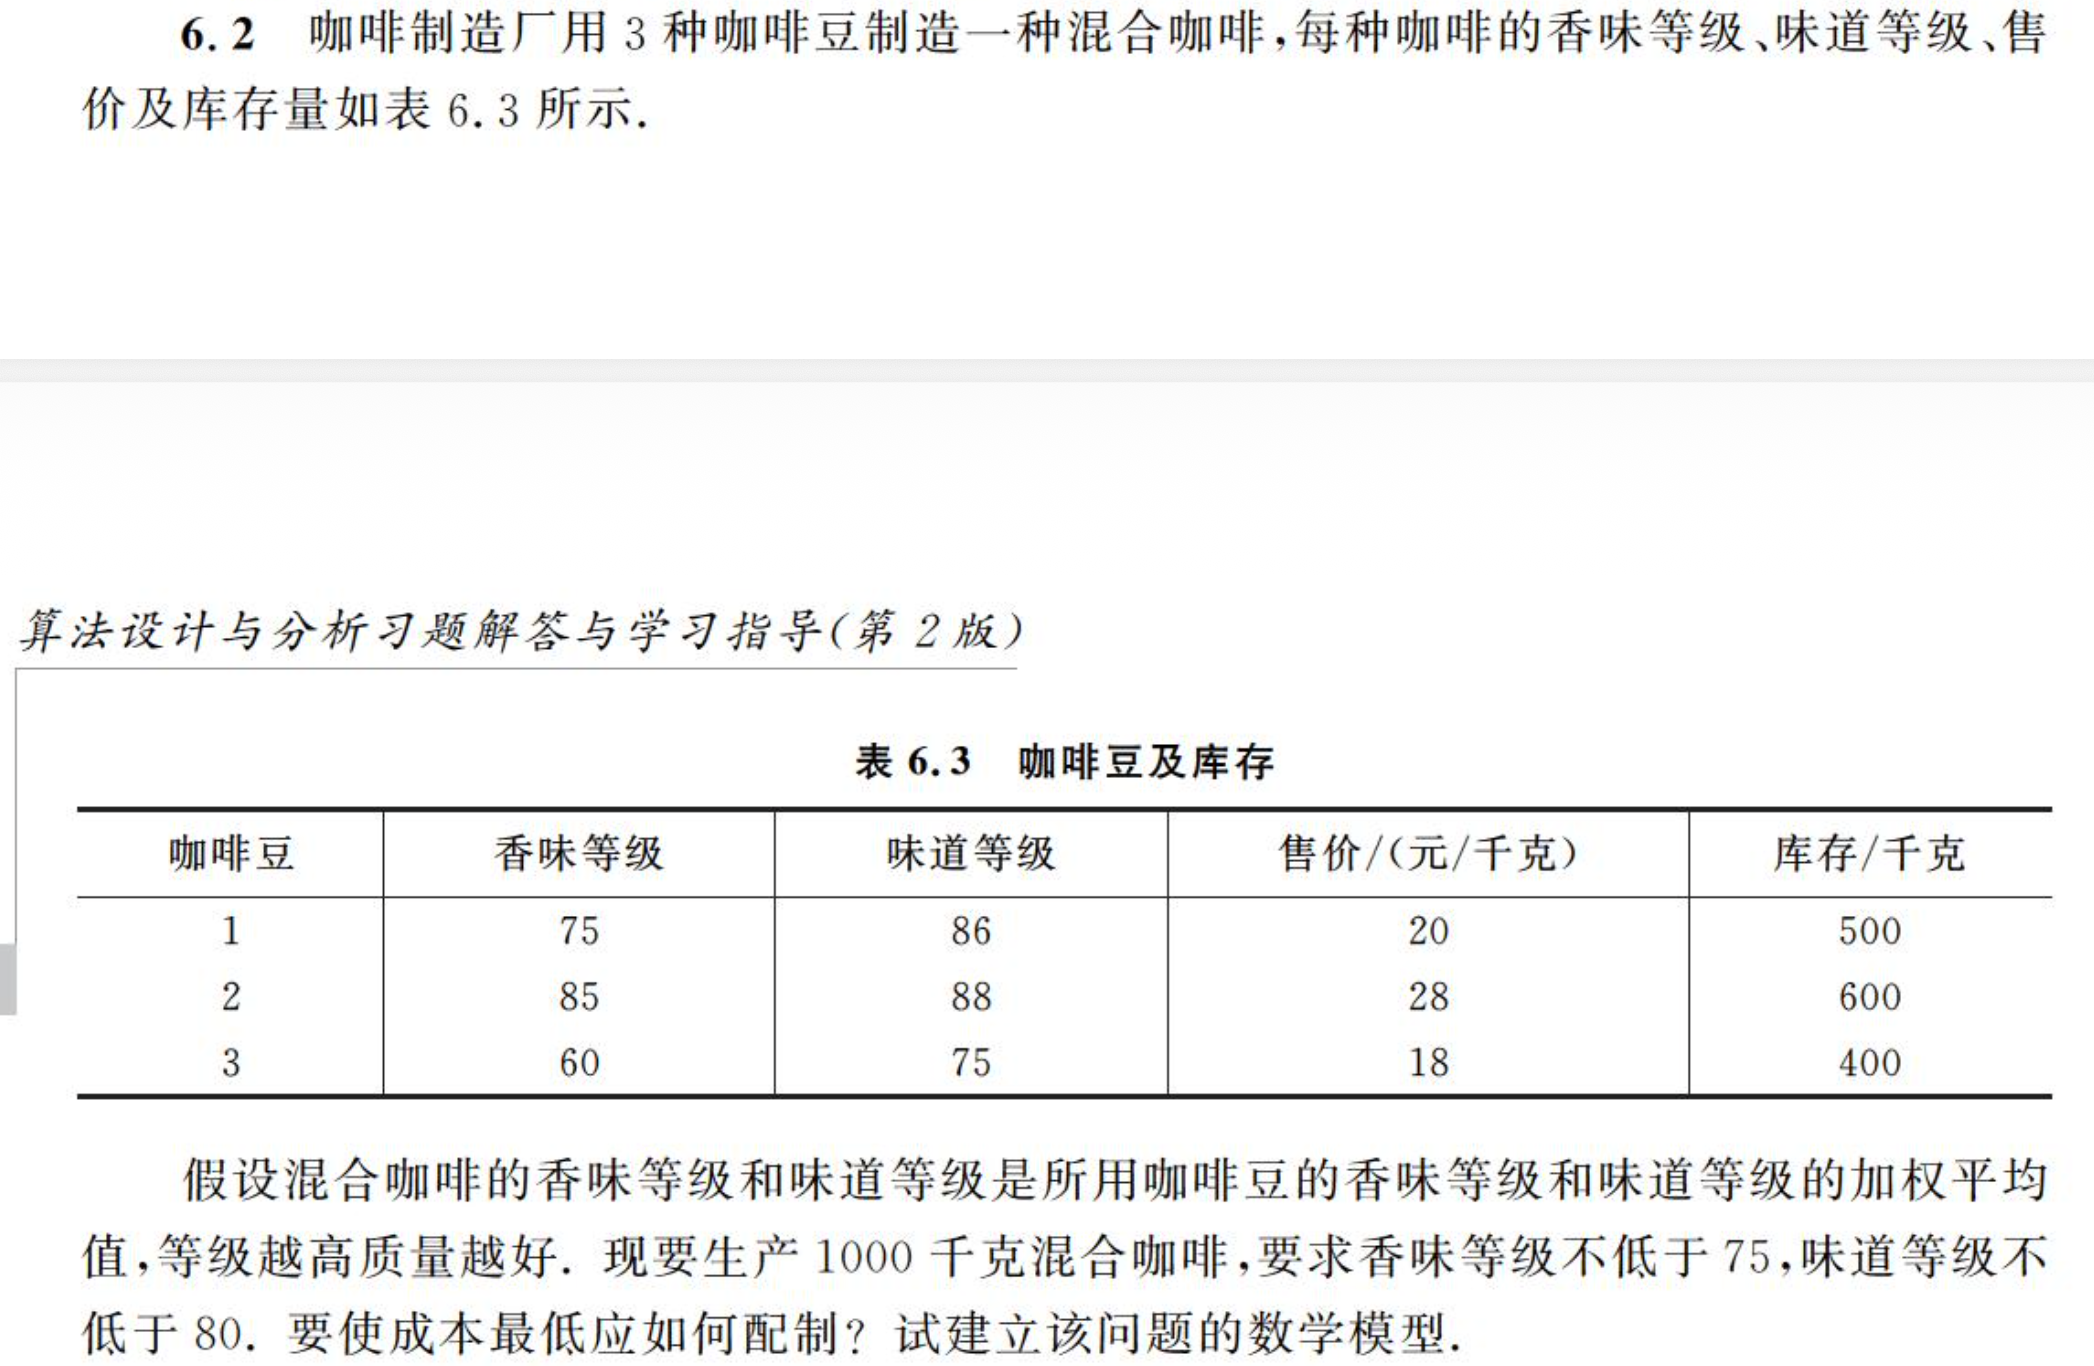
\includegraphics[width=0.6\textwidth]{problems/6.2.png}
\end{center}
\end{problem}

\begin{solution}
设3种咖啡豆的比例分别为 $x_1, x_2, x_3$, 问题表述为：求 $min 20x_1+28x_2+18x_3$, s.t.
\begin{itemize}
    \item $75x_1+85x_2+60x_3 \geq 75 $
    \item $86x_1+88x_2+75x_3 \geq 80 $
    \item $x_1+x_2+x_3 = 1 $
    \item $1000x_1 \leq 500 $
    \item $1000x_2 \leq 600 $
    \item $1000x_3 \leq 400 $
    \item $x_1, x_2, x_3 \geq 0$
\end{itemize}
\end{solution}

\begin{problem}
\begin{center}
    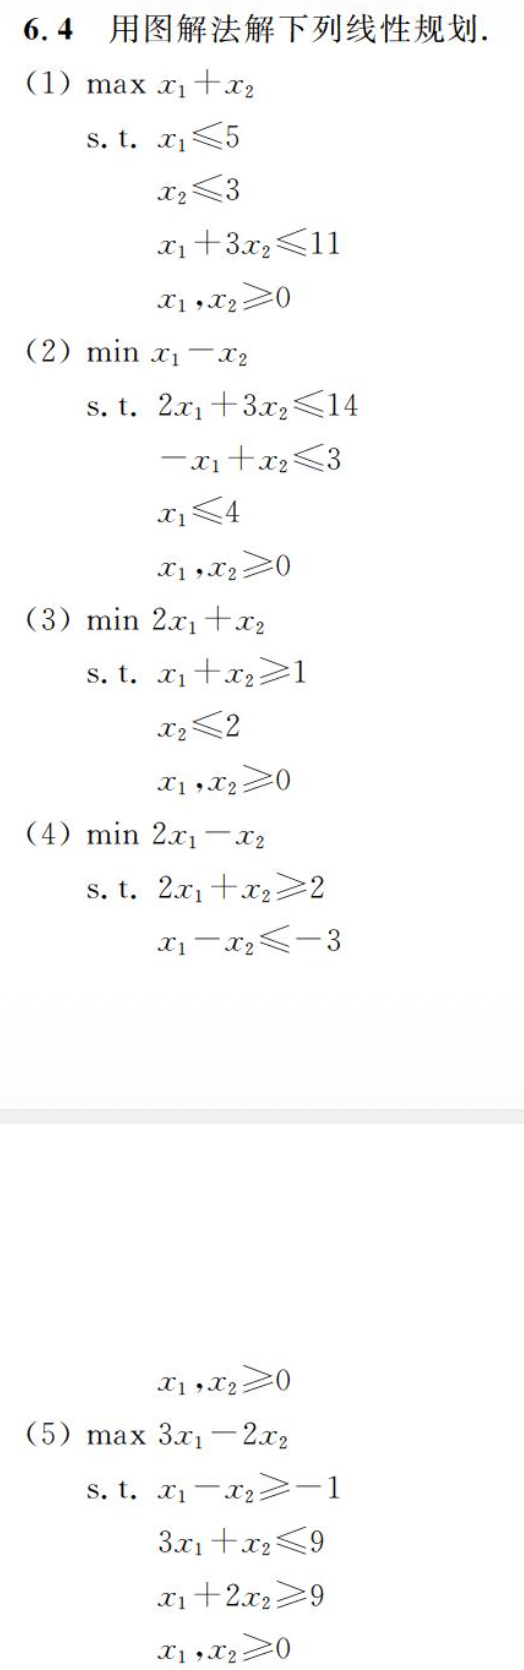
\includegraphics[width=0.3\textwidth]{problems/6.4.png}
\end{center}
\end{problem}

\begin{solution}
(1)
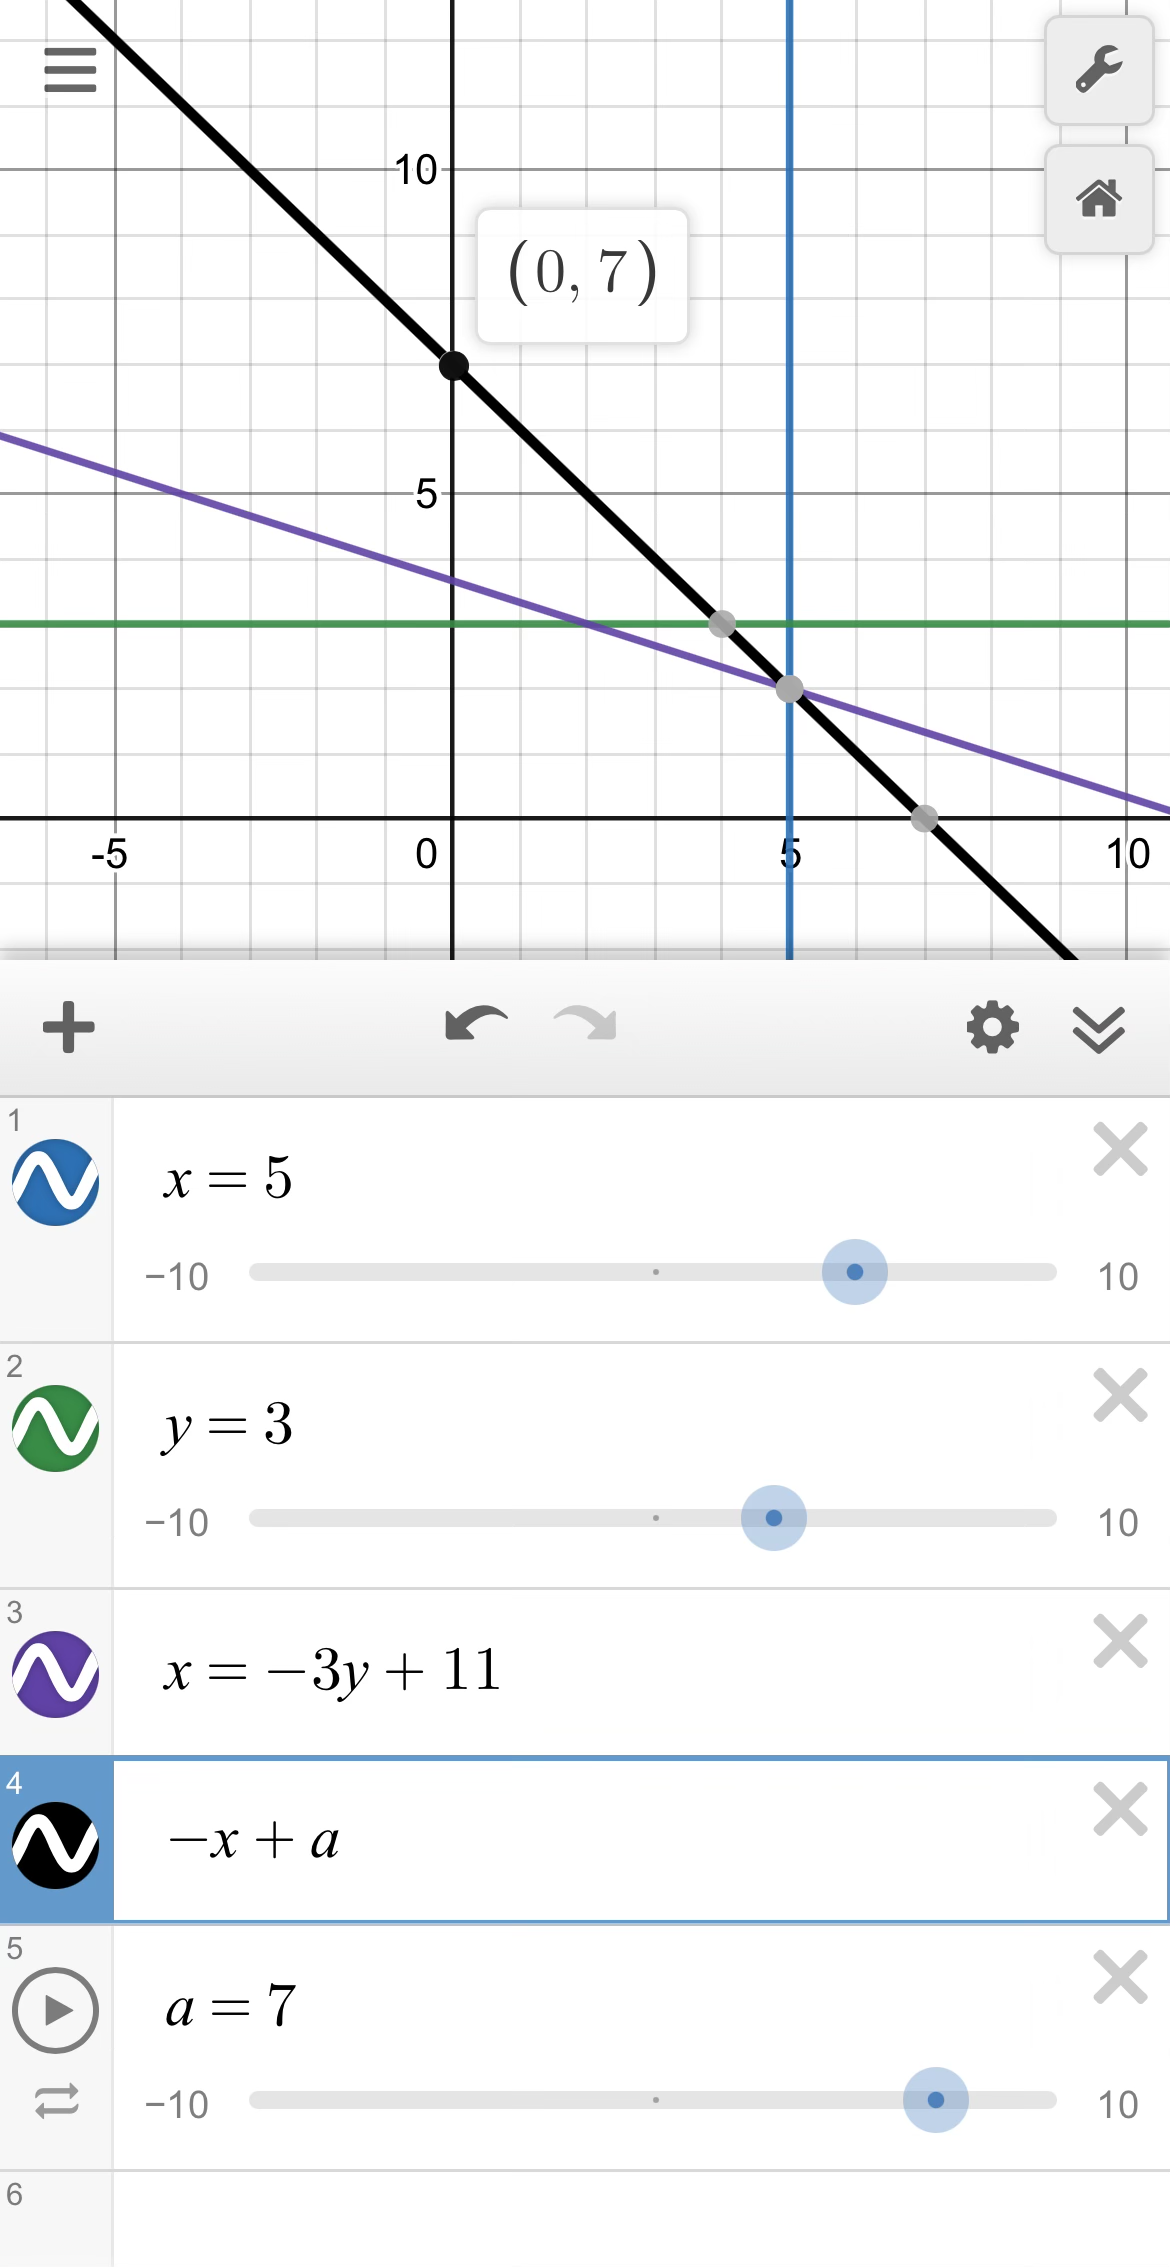
\includegraphics[width=0.3\textwidth]{problems/6.4-1.png} \\
由图可知，最大值为7. \\
(3)
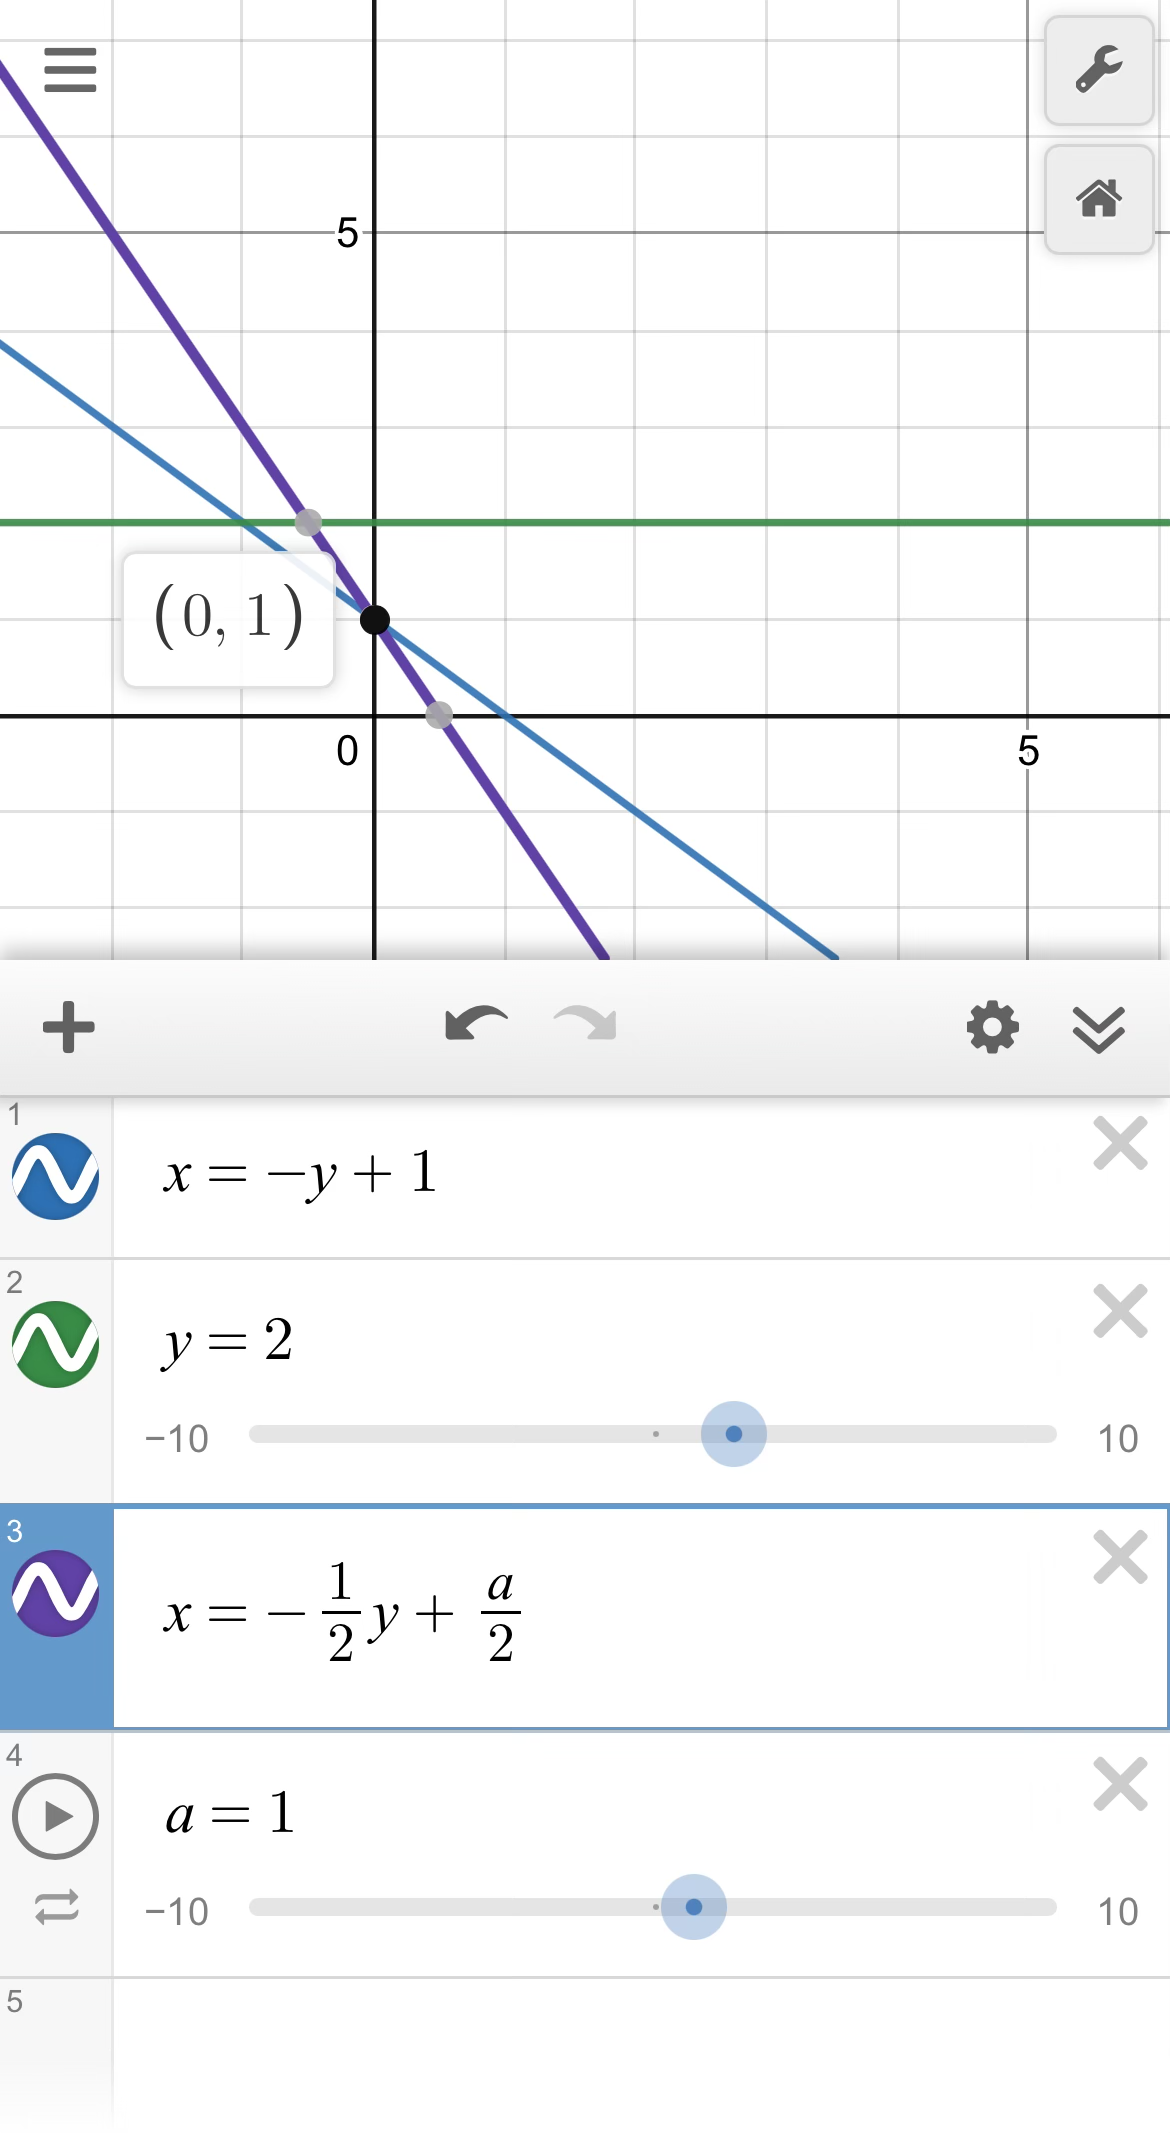
\includegraphics[width=0.3\textwidth]{problems/6.4-3.png} \\
由图可知，最小值为2.
\end{solution}

\begin{problem}
\begin{center}
    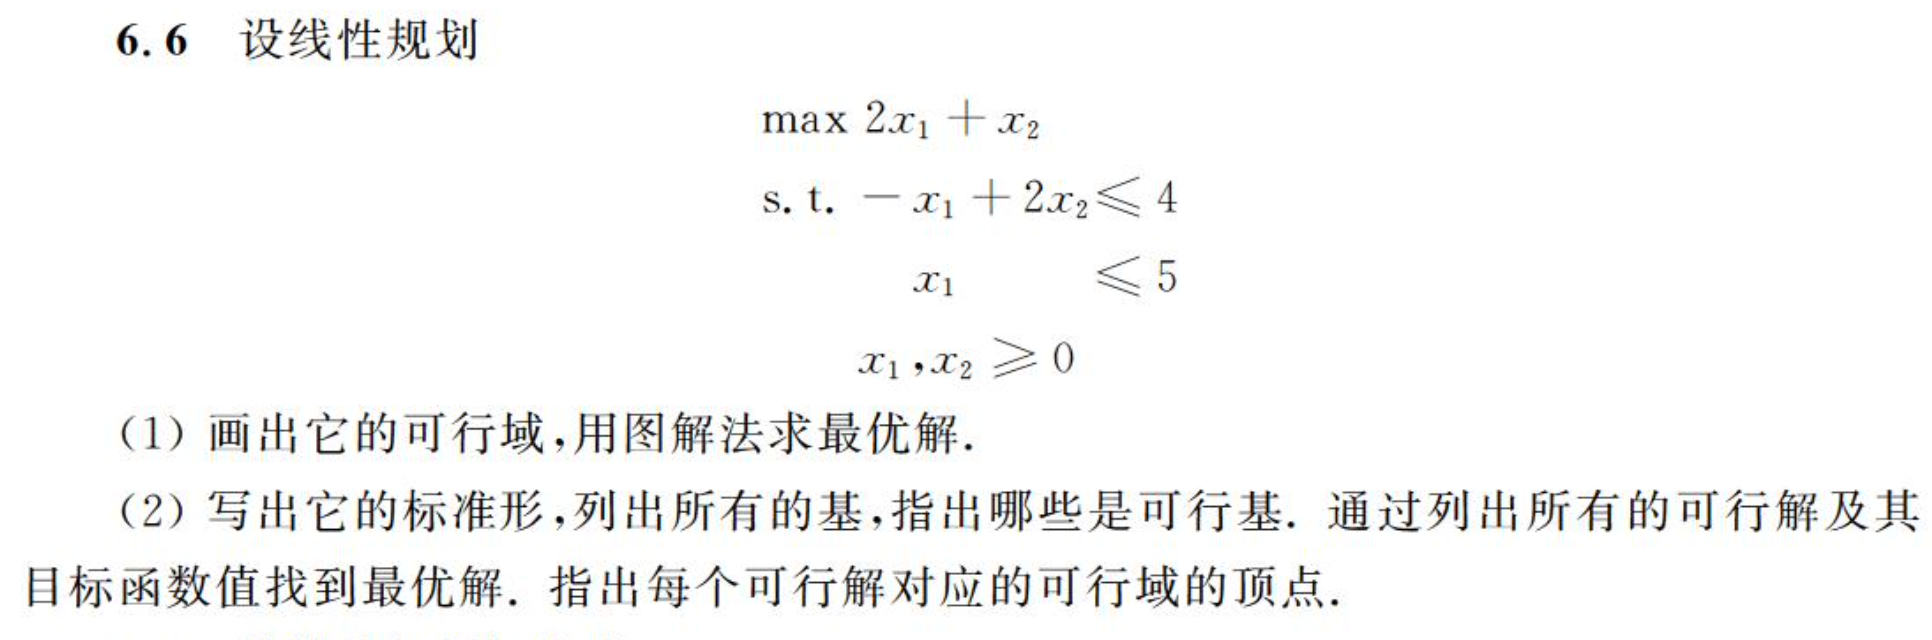
\includegraphics[width=0.6\textwidth]{problems/6.6.png}
\end{center}
\end{problem}

\begin{solution}
(1)
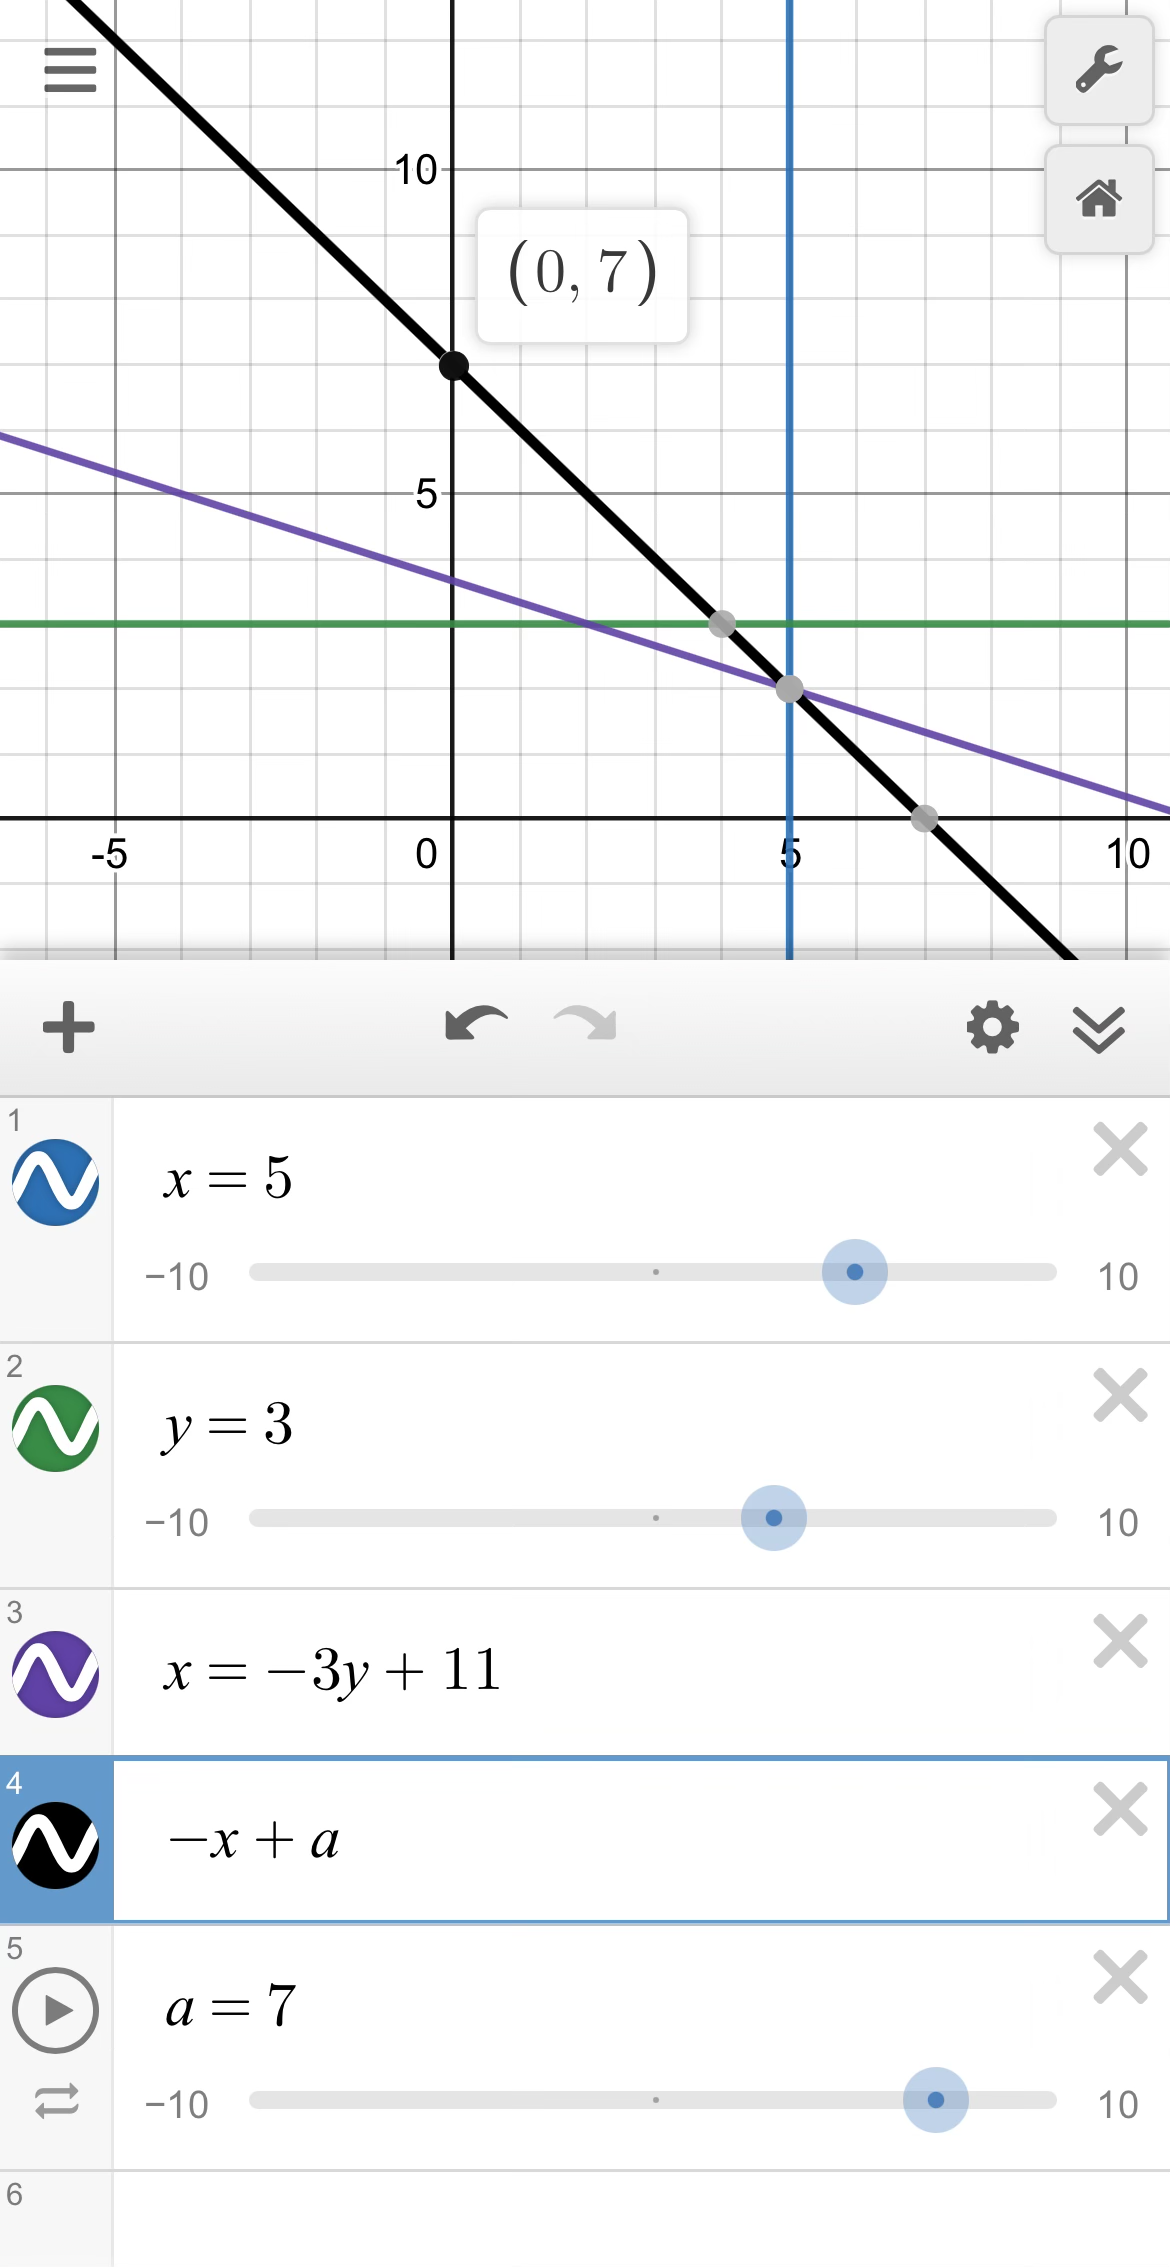
\includegraphics[width=0.3\textwidth]{problems/6.4-1.png} \\
由点 $(0, 0), (0, 2), (5, 4.5), (5, 0) $包围点四变形区域是该线性规划的可行域，由图知最大值为14.5，最优解是点 $(5, 4.5)$. \\
(2)
引入松弛变量 \(x_3,x_4\ge 0\)，则原问题可化为标准形
\[
\max \; 2x_1+x_2
\]
\[
\text{s.t.}\quad 
\begin{cases}
-x_1+2x_2+x_3=4,\\
x_1+x_4=5,\\
x_1,x_2,x_3,x_4\ge 0.
\end{cases}
\]

写成矩阵形式为
\[
A=
\begin{pmatrix}
-1 & 2 & 1 & 0\\
1 & 0 & 0 & 1
\end{pmatrix},
\qquad
b=
\begin{pmatrix}
4\\
5
\end{pmatrix},
\qquad
c=
\begin{pmatrix}
2\\
1\\
0\\
0
\end{pmatrix}.
\]

其中各列向量分别为
\[
a_1=\binom{-1}{1},\quad
a_2=\binom{2}{0},\quad
a_3=\binom{1}{0},\quad
a_4=\binom{0}{1}.
\]


由于约束方程有 \(2\) 个，所以基由 \(A\) 的任意两个线性无关列组成。考察所有二元组合：

\[
B_{12}=(a_1,a_2),\quad
B_{13}=(a_1,a_3),\quad
B_{14}=(a_1,a_4),\quad
B_{23}=(a_2,a_3),\quad
B_{24}=(a_2,a_4),\quad
B_{34}=(a_3,a_4).
\]

其中
\[
\det(a_2,a_3)=
\begin{vmatrix}
2 & 1\\
0 & 0
\end{vmatrix}
=0,
\]
故 \(B_{23}\) 不是基。

其余
\[
\{a_1,a_2\},\ \{a_1,a_3\},\ \{a_1,a_4\},\ \{a_2,a_4\},\ \{a_3,a_4\}
\]
都是基。


\begin{enumerate}
    \item 基 \(B_{12}=\{a_1,a_2\}\)

    取非基变量 \(x_3=x_4=0\)，则
    \[
    \begin{cases}
    -x_1+2x_2=4,\\
    x_1=5.
    \end{cases}
    \]
    解得
    \[
    x_1=5,\quad x_2=\frac{9}{2}.
    \]
    因而基本解为
    \[
    (x_1,x_2,x_3,x_4)=\left(5,\frac92,0,0\right).
    \]
    该解非负，因此是可行基。

    对应原问题中的顶点为
    \[
    (5,4.5).
    \]

    \item 基 \(B_{13}=\{a_1,a_3\}\)

    取非基变量 \(x_2=x_4=0\)，则
    \[
    \begin{cases}
    -x_1+x_3=4,\\
    x_1=5.
    \end{cases}
    \]
    解得
    \[
    x_1=5,\quad x_3=9.
    \]
    因而基本解为
    \[
    (x_1,x_2,x_3,x_4)=(5,0,9,0).
    \]
    该解非负，因此是可行基。

    对应原问题中的顶点为
    \[
    (5,0).
    \]

    \item 基 \(B_{14}=\{a_1,a_4\}\)

    取非基变量 \(x_2=x_3=0\)，则
    \[
    \begin{cases}
    -x_1=4,\\
    x_1+x_4=5.
    \end{cases}
    \]
    解得
    \[
    x_1=-4,\quad x_4=9.
    \]
    因而基本解为
    \[
    (x_1,x_2,x_3,x_4)=(-4,0,0,9).
    \]
    因 \(x_1<0\)，故该基不是可行基。

    \item 基 \(B_{24}=\{a_2,a_4\}\)

    取非基变量 \(x_1=x_3=0\)，则
    \[
    \begin{cases}
    2x_2=4,\\
    x_4=5.
    \end{cases}
    \]
    解得
    \[
    x_2=2,\quad x_4=5.
    \]
    因而基本解为
    \[
    (x_1,x_2,x_3,x_4)=(0,2,0,5).
    \]
    该解非负，因此是可行基。

    对应原问题中的顶点为
    \[
    (0,2).
    \]

    \item 基 \(B_{34}=\{a_3,a_4\}\)

    取非基变量 \(x_1=x_2=0\)，则
    \[
    \begin{cases}
    x_3=4,\\
    x_4=5.
    \end{cases}
    \]
    因而基本解为
    \[
    (x_1,x_2,x_3,x_4)=(0,0,4,5).
    \]
    该解非负，因此是可行基。

    对应原问题中的顶点为
    \[
    (0,0).
    \]
\end{enumerate}

所以，可行基共有四个：
\[
\{a_1,a_2\},\quad \{a_1,a_3\},\quad \{a_2,a_4\},\quad \{a_3,a_4\}.
\]

对应的可行基本解分别为
\[
\left(5,\frac92,0,0\right),\quad
(5,0,9,0),\quad
(0,2,0,5),\quad
(0,0,4,5).
\]

对应原问题可行域的顶点分别为
\[
\left(5,\frac92\right),\quad
(5,0),\quad
(0,2),\quad
(0,0).
\]

最优解为
\[
x_1^*=5,\qquad x_2^*=4.5,
\]
最优值为
\[
z^*=14.5.
\]
\end{solution}

\begin{problem}
\begin{center}
    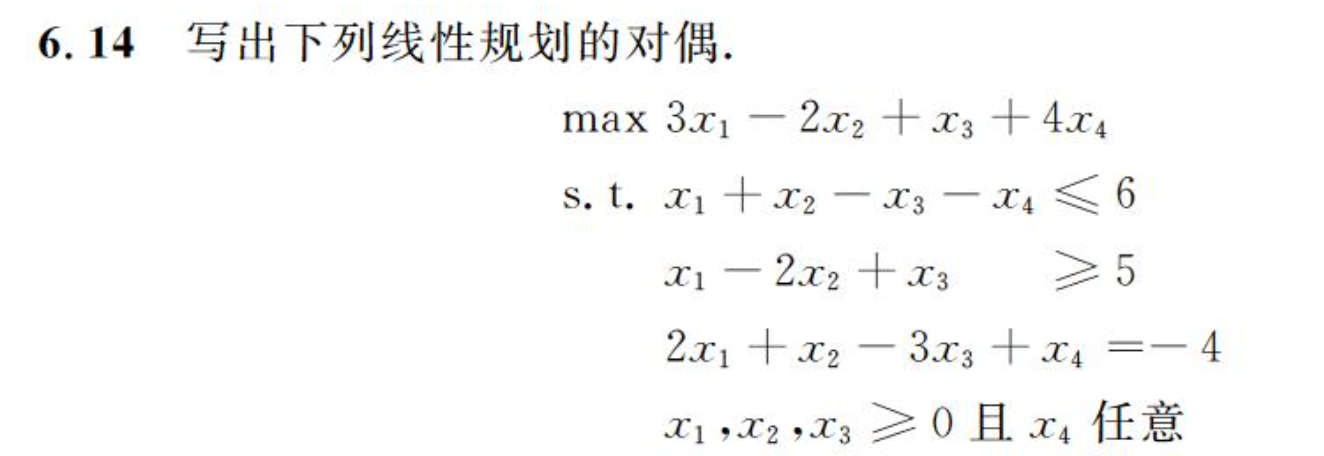
\includegraphics[width=0.6\textwidth]{problems/6.14.png}
\end{center}
\end{problem}

\begin{solution}
原问题是最大化问题，因此各约束对应的对偶变量满足：
\[
\begin{cases}
y_1 \ge 0, & \text{对应 } \le \text{ 型约束},\\
y_2 \le 0, & \text{对应 } \ge \text{ 型约束},\\
y_3 \text{ 自由}, & \text{对应 } = \text{ 型约束}.
\end{cases}
\]

原问题右端向量为
\[
b=\begin{pmatrix}6\\5\\-4\end{pmatrix},
\]
故对偶问题的目标函数为
\[
\min \; 6y_1+5y_2-4y_3.
\]

原问题各变量的列向量分别为
\[
a_1=\begin{pmatrix}1\\1\\2\end{pmatrix},\quad
a_2=\begin{pmatrix}1\\-2\\1\end{pmatrix},\quad
a_3=\begin{pmatrix}-1\\1\\-3\end{pmatrix},\quad
a_4=\begin{pmatrix}-1\\0\\1\end{pmatrix}.
\]

由于
\[
c=\begin{pmatrix}3\\-2\\1\\4\end{pmatrix},
\]
并且原问题中
\[
x_1,x_2,x_3\ge 0,\qquad x_4 \text{ 自由},
\]
所以对偶约束分别为
\[
a_1^T y \ge 3,\qquad
a_2^T y \ge -2,\qquad
a_3^T y \ge 1,\qquad
a_4^T y = 4.
\]

展开后得到
\[
\begin{cases}
y_1+y_2+2y_3 \ge 3,\\
y_1-2y_2+y_3 \ge -2,\\
-y_1+y_2-3y_3 \ge 1,\\
-y_1+y_3 = 4.
\end{cases}
\]

因此，对偶问题为
\[
\text{对偶 }(D)\!:\quad
\min \; 6y_1+5y_2-4y_3
\]
\[
\text{s.t.}\quad
\begin{cases}
y_1+y_2+2y_3 \ge 3,\\
y_1-2y_2+y_3 \ge -2,\\
-y_1+y_2-3y_3 \ge 1,\\
-y_1+y_3 = 4,\\
y_1\ge 0,\quad y_2\le 0,\quad y_3\ \text{任意}.
\end{cases}
\]
\end{solution}

\end{document}